\graphicspath{{chapters/contents/sessio_04/images/}}
\chapter{Sessió 4 (05/10/2026). Els àtoms existeixen. Quadern de laboratori}

\section{Te'n recordes del volcà?}

Te'n recordes de l'experiment del volcà que fèiem de petits? Era divertit: barrejaves unes quantes coses, començava a sortir escuma per tot arreu i durant uns segons allò semblava bastant més emocionant que una classe normal.

Apreníem alguna cosa? Bé, com a mínim una: que podies ajuntar dues substàncies, barrejar-les amb aigua i aconseguir que passés una cosa completament diferent.

Mmm. Interessant.

També és una bona manera de continuar estirant del fil. Repetirem l'experiment del volcà, però aquesta vegada amb una mica més de ciència, bastant més de control i amb la intenció d'entendre què està passant de debò.

\section{El treball de laboratori}

Aquí ens posem seriosos.

El treball de laboratori ha de ser rigorós i molt acurat. Segur que no t'imagines fent-te una anàlisi de sang i trobant-te al laboratori tots els tubs de mostres escampats per sobre la taula mentre algú s'empassa un Yatekomo i mira TikToks.

Quan entrem al laboratori posem el cervell en \emph{mode laboratori}: serietat, ordre, atenció, gestos curosos i paciència. Ens fixem en els detalls i intentem que tot sigui tan exacte com sigui possible.

Del treball d'un laboratori pot dependre comprovar la resistència del ciment d'un pont, detectar una malaltia. En alguns experiments s’hi han invertit molts diners o hi pots haver dedicat moltíssimes hores de feina, i tot es pot arruïnar simplement per no haver anat amb prou cura.

Això és seriós.

\section{Els rituals}

Per arribar a l'estat que necessitem, els rituals ajuden molt. Li diuen al cervell: ``Ei, ara toca parar atenció''.

Rentar-se les mans, posar-se l'equip de seguretat, preparar el material, conèixer bé les instruccions i fer cada pas en l'ordre correcte.

Hi ha molta gent a qui el treball de laboratori li encanta. Quan comences a fer-ho bé, enganxa una mica. Si ets una mica descuidat o descuidada, en canvi, pot ser frustrant: en química no funciona gaire això de ``ho faig de qualsevol manera i després ja veurem com ho arreglo''. Quan l'experiment s'ha fet malament, normalment no hi ha un botó de desfer.

A la cuina existeix el concepte de \emph{mise en place}: abans de començar es col·loca tot el que necessitarem, es repassa visualment la llista i ens assegurem que no falta res que pugui espatllar l'experiment.

Comencem per aquí.

Mira la imatge, col·loca tot el material tal com apareix i assegura't que ho tens tot. Respira, concentra't i de seguida podràs començar a treballar.

\begin{figure}[H]
    \centering
    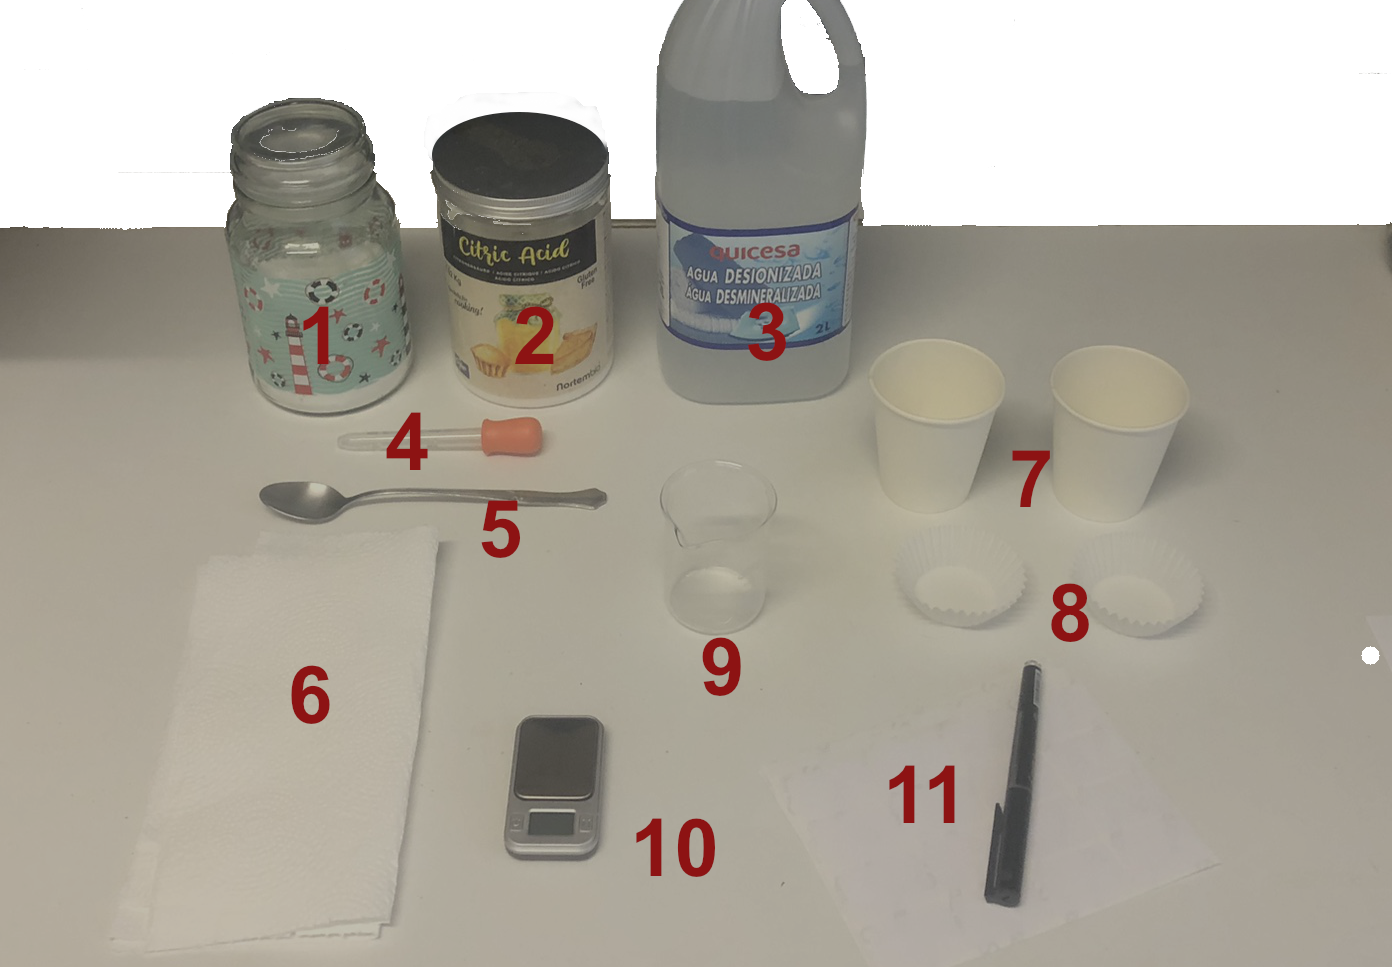
\includegraphics[width=0.80\linewidth]{setup.png}
    \caption{Comprova que coneixes i saps utilitzar correctament cadascun dels objectes.  Imatge creada per l’autor, CC BY 4.0.}
\end{figure}

\vfill
\newpage

Repassa aquesta llista i identifica aquests objectes a la teva taula de treball.

\begin{enumerate}
    \item Bicarbonat de sodi
    \item Àcid cítric
    \item Aigua destil·lada
    \item Comptagotes
    \item Cullereta
    \item Uns quants papers de cuina
    \item Dos gots de paper
    \item Dos motlles de magdalena
    \item Un recipient de vidre (vas de precipitats)
    \item Una balança digital amb precisió de dècimes de gram
    \item Etiquetes adhesives i un bolígraf
\end{enumerate}


\section{Però abans... seguretat}

Avui estem treballant amb substàncies que també podem trobar en una cuina. Però alerta: això no vol dir que al laboratori tot funcioni així.

Depenent del que estiguem fent podem necessitar ulleres de seguretat, guants, bata i, si cal, una campana extractora, una màscara antipols o protecció davant de determinats gasos.

En aquesta pràctica el risc és petit, però treballarem des del principi amb bons hàbits de laboratori.

\begin{itemize}
    \item Segueix les instruccions en ordre i assegura't que les entens.
    \item Obre un pot cada vegada. Tanca'l i torna'l a deixar al seu lloc després d'utilitzar-lo.
    \item Fes el mateix amb la resta de materials: pots, comptagotes, culleres i recipients.
    \item Mantén sempre la superfície de treball neta. Si es vessa alguna cosa, neteja-la immediatament. No continuïs treballant en un abeurador d'ànecs, home.
    \item Al laboratori no es menja ni es beu res, ni el que portes de casa ni, encara menys, allò amb què estàs treballant.
    \item Tingues a prop un lloc on et puguis rentar bé si arriba a fer falta.
    \item Assegura't que saps utilitzar la balança i fer correctament la tara.
    \item Quan acabis l'experiment, neteja a mesura que deixis de necessitar cada cosa. Deixa tot el material ben guardat, tancat i ordenat. L'àrea de treball ha de quedar impecable.
    \item Utilitza les etiquetes. No confiïs en això de ``ja me'n recordaré després''.
\end{itemize}

En resum: el laboratori pot ser divertit i enganxar bastant, però no perdem mai de vista que també exigeix molta responsabilitat.

\section{Ara sí. Comencem}

\subsection{Pas 1. Mesurem l'aigua}

Fes la tara de la balança amb el got de paper buit.

Segons el teu grup, mesura la quantitat d'aigua que indica la fitxa:

\[
50\ \text{g d'aigua}
\]
o bé
\[
60\ \text{g d'aigua}
\]

Fixa't que aquests valors coincideixen aproximadament amb els mil·lilitres:

\[
50\ \text{g} \approx 50\ \text{mL}
\]
\[
60\ \text{g} \approx 60\ \text{mL}
\]

No és casualitat que hàgim triat aquestes quantitats.

Pots utilitzar el comptagotes per afegir o treure aigua i ser més precís. Si et passes una mica, gairebé és millor treure'n una mica i tornar a afegir gota a gota. 
També pots deixar una mica d'aigua de reserva al vas de precipitats.



\vfill
\newpage

\subsection{Pas 2. Mesurem l'àcid cítric}

Per a tots els grups, mesura exactament:
\[
10,0\ \text{g d'àcid cítric}
\]

Utilitza un motlle de magdalena i recorda fer la tara de la balança abans de pesar.

\subsection{Pas 3. Afegim l'àcid}

Aboca completament l'àcid cítric dins de l'aigua.

Assegura't que no en queda enganxat al motlle i que no en perds gens pel camí.

\subsection{Pas 4. Mesurem el bicarbonat}

En l'altre motlle de magdalena, pesa la quantitat de bicarbonat de sodi que correspon al teu grup.

Segons la fitxa hauràs de pesar:

\[
13,1\ \text{g}
\]
o bé
\[
15,0\ \text{g}
\]
Recorda, una altra vegada, fer la tara de la balança.

\subsection{Pas 5. Etiquetem la dissolució.}

Anota en una etiqueta les proporcions d’aigua i bicarbonat que has utilitzat i enganxa-la al got. La quantitat d’àcid cítric ja la sabem: sempre és de 10 g.

\subsection{Pas 6. Preparem la dissolució}

Barreja molt bé el recipient on has posat l'àcid cítric i l'aigua.

Ens interessa especialment que no es perdi res de la mescla. Si es vessa líquid o en queda fora del recipient, després ja no sabrem exactament què estem mesurant.
Sí, a partir d’ara ens obsessionarem una mica amb això.

Quan estigui ben barrejat, treu la cullera. Abans, dona-li el típic copet perquè totes les gotes tornin al recipient.



\vfill
\newpage

\subsection{Pas 7. El volcà, per fi... però una mica esquifit.}

Ara sí.

Agafa petites porcions de bicarbonat amb la punta de la cullera i afegeix-les molt a poc a poc. Veuràs que la dissolució comença a bombollejar com una banyera d’hidromassatge.

Després de cada petita porció, espera que la reacció baixi. Pots comptar fins a 20 abans d'afegir-ne més.

No tinguis pressa. Som al laboratori.

Si afegeixes massa bicarbonat de cop, la mescla pot vessar-se i l'experiment deixarà de funcionar bé. Un bon indicador és la teva pròpia mà: si comences a notar-hi esquitxades, probablement vas massa ràpid.

\subsection{Pas 8. Esperem que acabi la reacció}

Quan hagis afegit tot el bicarbonat, continua remenant suaument.

No remenis més fort per acabar abans. Si t'avorreixes, abans de convertir el recipient en una centrifugadora improvisada, demana a algú que et substitueixi.

Arribarà un moment en què, encara que remenis, ja no apareixeran bombolles.

Pot trigar aproximadament un quart d'hora.

\subsection{Pas 9. Pesem el que queda}

Ja ho tenim.

Hem fet el volcà, però aquesta vegada molt més lentament i de manera controlada.

Treu la cullera i sacseja-la suaument perquè no quedi ni una gota de líquid enganxada.

Ara fes la tara de la balança amb el got de paper que havia quedat buit.

Després pesa el recipient que conté el líquid final.

\vfill
\newpage

\section{I ara què ha passat?}

Suma la massa inicial de:

\begin{itemize}
    \item l'aigua,
    \item l'àcid cítric,
    \item el bicarbonat de sodi.
\end{itemize}

Compara aquest valor amb la massa del líquid que queda al final.

La diferència hauria de ser d'aproximadament:

\[
6,9\ \text{g}
\]

Probablement serà una mica menys. En un experiment real sempre es pot perdre alguna gota, quedar alguna substància enganxada a un recipient o produir-se petits errors de mesura.

Però, si el treball s'ha fet amb cura, el resultat hauria de quedar bastant a prop.

I aquí arriba la part interessant:

\textbf{en els tres casos, la mescla ha perdut aproximadament 6,9 grams.}

Discutirem aquest resultat al full de solucions.

\section{Però abans d'explicar-ho... pensem-hi una mica}

Tots els grups heu afegit:

\begin{itemize}
    \item \(10\ \text{g}\) d'àcid cítric;
    \item alguns, \(50\ \text{g}\) d'aigua i altres, \(60\ \text{g}\);
    \item alguns, \(13,1\ \text{g}\) de bicarbonat de sodi i altres, \(15,0\ \text{g}\).
\end{itemize}

Per tant, les quantitats inicials no eren exactament les mateixes.

I, tot i això, si l'experiment s'ha fet amb prou cura, tots els grups heu perdut aproximadament la mateixa quantitat d'``alguna cosa'' quan la reacció ha acabat:

\[
6,9\ \text{g}
\]

Què ens diu això?

Doncs, ni més ni menys, ens dona una pista més (entre moltes altres) que els àtoms existeixen.

\section{Àtoms com peces de LEGO}

Els àtoms reaccionen en proporcions molt concretes, una mica com les peces de LEGO.

Imagina que tens 10 peces vermelles i 15 peces blaves i vols construir torres formades sempre per una peça vermella a sota i una peça blava a sobre.

Podràs construir 10 torres.

I et sobraran 5 peces blaves.

No importa que en tinguessis 12, 15 o 200: quan s'acaben les peces vermelles, ja no pots construir més torres d'aquell tipus.

Aquí està passant una cosa semblant.

A les solucions de l’activitat ho veurem com ho veu la química.

\section{Annex.}

\begin{table}[h]
\centering
\caption{Fitxa de proporcions per als grups}
\small
\begin{tabular}{c|cc}
\hline
\textbf{Grup} & \textbf{Aigua (g)} & \textbf{Bicarbonat (g)} \\
\hline
1 & 50 & 13,1 \\
2 & 50 & 15,0 \\
3 & 60 & 13,1 \\
4 & 60 & 15,0 \\
\hline
\end{tabular}

\vspace{0.3em}
\footnotesize
\textit{En tots els grups s'utilitzen 10,0 g d'àcid cítric.}
\end{table}